\section{Visualising Process Model Forecasts}\label{sec:visualisation}


% as has been shown the prediction is nice but it is difficult to derive the insignts 
% definition of the visualization
% humans cannot comprehend the results and we need visualzation 
% (new functions on vis that ar enot mentioned before should be mentioned?)

%%%
% outline:
% 1. requirements
% 2. design (and what supports design)
% 3. system overview
%%%
The evaluation Section~\ref{sec:experiment} has shown a good performance of the prediction algorithms for the process model forecasts. To that end, deriving insights from such predicted data remains a difficult task for the analyst. In this section we present the design of visualization system that aids analysts in exploration of the past and future of the processes.

We designed a Process Change Exploration (PCE) system to support the interpretation of the process model forecasts. In order to design the system we first established requirements for the visualization based on the related literature and experience working with event sequence data. We then designed several prototypes, that after several rounds of discussions matured into the implemented visualization system.

To derive the requirements we focus on the requirements of process mining analysis with respect to process forecasting and visualization principles. The authors of~\cite{DBLP:conf/bpm/PollPRRR18} discuss the opportunities for process forecasting. They describe that the possible utility of the process forecasting is an understanding the incremental changes or adaptations that happen to the process model into the future. In designing an exploitative visualization system, we followed the "Visual Information-Seeking Mantra:"~\emph{overview first, zoom and filter, then details-on-demand}~\cite{DBLP:conf/vl/Shneiderman96}. 
(maybe talk about tasks? not requirements)
Thus, we expect our system to assist in:

\begin{requidescr}
	\item[Identify process adaptations:\namedlabel{req:adaptation}] The visualisation system should assist the user in identifying the changes changes that happen in the process model;
	\item[Allow for interactive exploration:\namedlabel{req:interactive}] The user should be able to follow the visual information-seeking principles;
	
\end{requidescr} % CUSTOM from CDC, with love :)





\begin{figure}
	\centering
	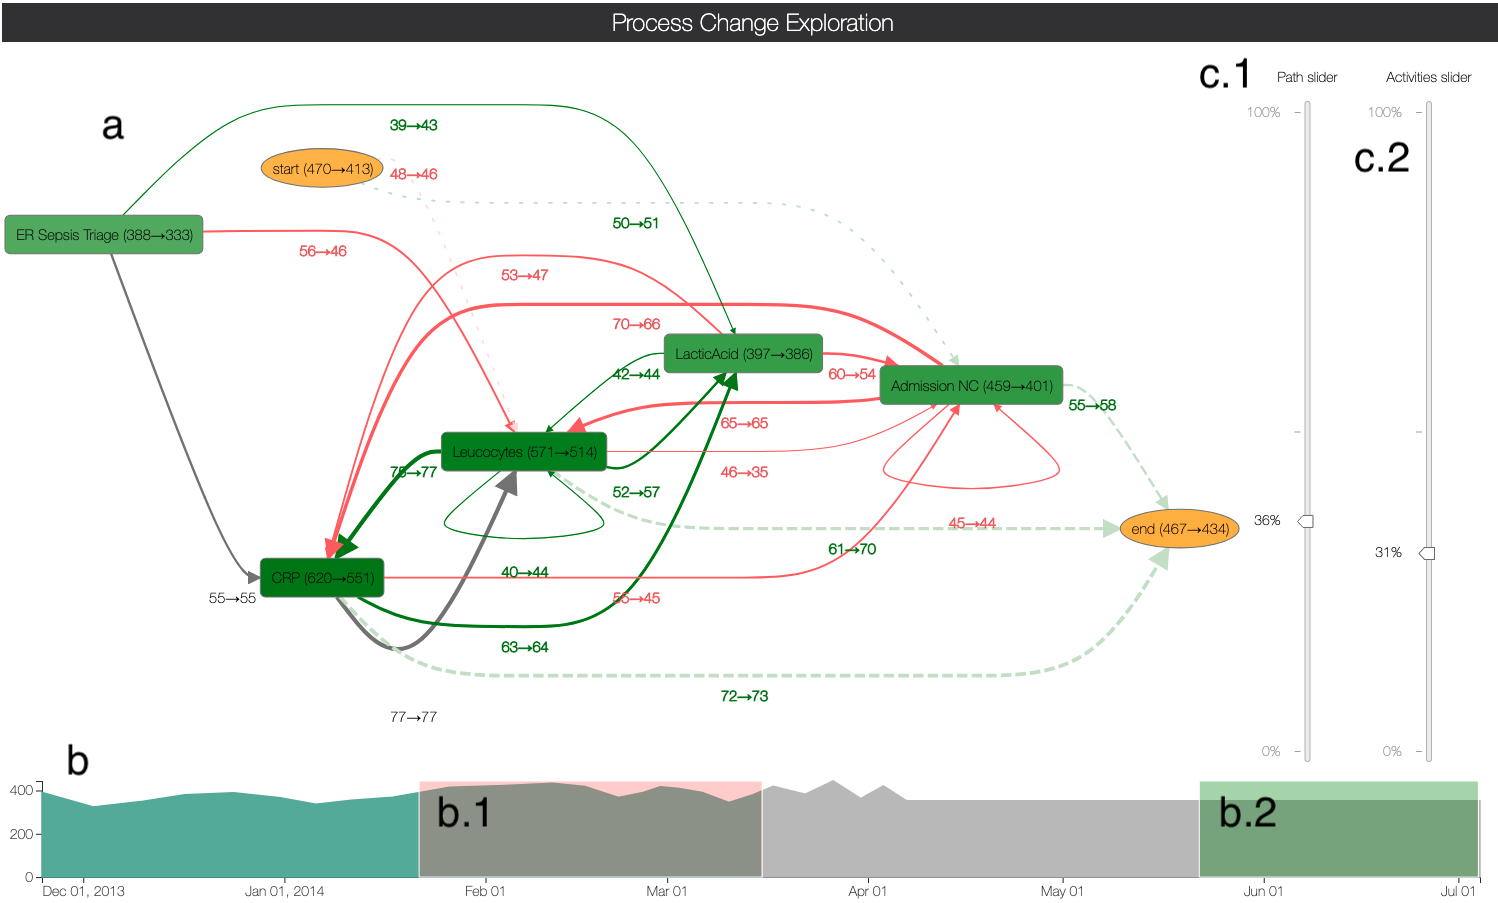
\includegraphics[width=\textwidth]{img/vis/vis-system-two-brushes.png}
	\caption{Process Change Exploration (PCE) system. The interactive system consists of three parts. Part b shows the timeline of the data (green region), and forecasted values (grey region). The user can brush one or two regions (in this b.1 and b.2) on this graph to see the filtered for that time range process model or a difference between two process models. The main view (a) represents the directly follows change graph that shows the difference between two brushed regions. The c.1 and c.2 are the usual filters on the number of paths and activities to aid simplification the visual representation} 
	\label{fig:vis-two-brushes}
\end{figure}

\begin{figure}
	\centering
	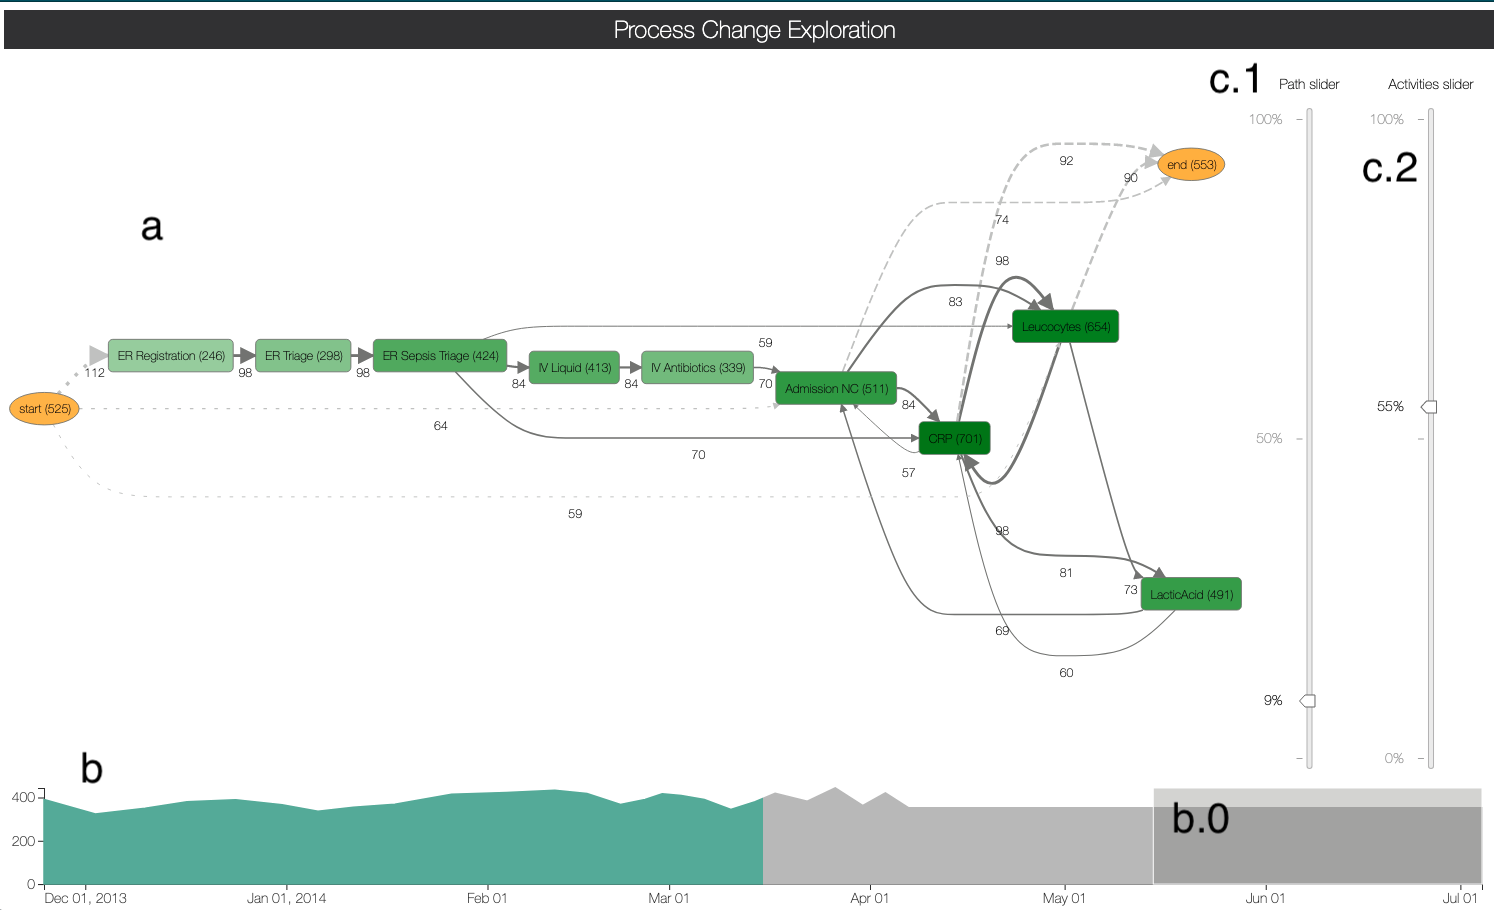
\includegraphics[width=\textwidth]{img/vis/vis-system-one-brush.png}
	\caption{Process Change Exploration (PCE) system. The interactive system consists of three parts. Part b shows the timeline of the data (green region), and forecasted values (grey region). The user can brush one time range (in this b.0) on this graph to see the filtered for that time range process model. The main view (a) represents the directly follows graph of that region. The c.1 and c.2 are the usual filters on the number of paths and activities to aid simplification the visual representation} 
	\label{fig:vis-one-brushes}
\end{figure}


\noindent\textbf{%
	User interface
} The Figure~\ref{fig:vis-two-brushes} displays the screenshot of the PCE visualization system. 
We improve upon the notion of Directly-Follows graph~\cite{leemans2019directly} that is widely used in process mining research and practice. We use the ideas from the version graph~\cite{DBLP:conf/grapp/KriglsteinR12} on how to represent the change between versions of the graph with coloring of the transitions. 

..... and so on

The interactive visualization system was implemented in D3.JS JavaScript visualization library.








